\let\negmedspace\undefined
\let\negthickspace\undefined
\documentclass[journal]{IEEEtran}
\usepackage[a5paper, margin=10mm, onecolumn]{geometry}
%\usepackage{lmodern} % Ensure lmodern is loaded for pdflatex
\usepackage{tfrupee} % Include tfrupee package

\setlength{\headheight}{1cm} % Set the height of the header box
\setlength{\headsep}{0mm}     % Set the distance between the header box and the top of the text

\usepackage{gvv-book}
\usepackage{gvv}
\usepackage{cite}
\usepackage{amsmath,amssymb,amsfonts,amsthm}
\usepackage{algorithmic}
\usepackage{graphicx}
\usepackage{textcomp}
\usepackage{xcolor}
\usepackage{txfonts}
\usepackage{listings}
\usepackage{enumitem}
\usepackage{mathtools}
\usepackage{gensymb}
\usepackage{comment}
\usepackage[breaklinks=true]{hyperref}
\usepackage{tkz-euclide} 
\usepackage{listings}

% \usepackage{gvv}                                        
\def\inputGnumericTable{}                                 
\usepackage[latin1]{inputenc}                                
\usepackage{color}                                            
\usepackage{array}                                            
\usepackage{longtable}                                       
\usepackage{calc}                                             
\usepackage{multirow}                                         
\usepackage{hhline}                                           
\usepackage{ifthen}                                           
\usepackage{lscape}
\begin{document}

\bibliographystyle{IEEEtran}
\vspace{3cm}


\renewcommand{\thefigure}{\theenumi}
\renewcommand{\thetable}{\theenumi}
\setlength{\intextsep}{10pt} % Space between text and floats


\numberwithin{equation}{enumi}
\numberwithin{figure}{enumi}
\renewcommand{\thetable}{\theenumi}

\title{Gate ME-2007}
\author{AI24BTECH11032 Shreyansh Sonkar
}
\maketitle
\renewcommand{\thefigure}{\theenumi}
\renewcommand{\thetable}{\theenumi}
\begin{enumerate}
\item The minimum  value of function $y=x^{2}$ in the interval $\sbrak{1,5}$ is 
\begin{multicols}{4}
    \begin{enumerate}
        \item $0$
        \item $1$
        \item $25$
        \item undefined
    \end{enumerate}
\end{multicols}
\bigskip
\item If a square matrix A is real and symmetric,then the eigenvalues 
\begin{enumerate}
        \item are always real
        \item are always real and positive 
        \item are always real and non-negative
        \item occurs in complex conjugate pairs
 \end{enumerate}
\bigskip
\item If $\phi\brak{x,y}$ and $\psi\brak{x,y}$ are function with continuous  second derivatives,then$\phi\brak{x,y}+i\psi\brak{x,y}$ can be expressed as an analytic function of $x+iy\brak{i=\sqrt{-1}}$,when
\begin{enumerate}
        \item $\frac{\partial\phi}{\partial x}=\frac{-\partial\psi}{\partial x};\frac{\partial\phi}{\partial y}=\frac{\partial\psi}{\partial y}$
        \item $\frac{\partial\phi}{\partial y}=\frac{-\partial\psi}{\partial x};\frac{\partial\phi}{\partial x}=\frac{\partial\psi}{\partial y}$
        \item $\frac{\partial^{2}\phi}{\partial x^{2}}+\frac{\partial^{2}\phi}{\partial y^{2}}=\frac{\partial^{2}\psi}{\partial x^{2}}+\frac{\partial^{2}\phi}{\partial y^{2}}=1$
        \item$\frac{\partial\phi}{\partial x}+\frac{\partial\phi}{\partial y}=\frac{\partial\psi}{\partial x}+\frac{\partial\psi}{\partial y}=0$
\end{enumerate}
\bigskip
\item The partial differential equation 
\begin{align*}
    \frac{\partial^{2}\phi}{\partial x^{2}}+\frac{\partial^{2}\phi}{\partial y^{2}}+\brak{\frac{\partial\phi}{\partial x}}+\brak{\frac{\partial\phi}{\partial y}}=0
\end{align*}
has
\begin{multicols}{2}
    \begin{enumerate}
        \item degree 1 and 2
        \item degree 1 and 1
        \item degree 2 and 1
        \item degree 2 and 2
    \end{enumerate}
\end{multicols}
\bigskip
\item Which of the following relationships is valid only for reversible processes undergone by a closed system of simple compressible substance $\brak{\text{neglect changes in kinetic and potential energy}}?$
\begin{multicols}{2}
    \begin{enumerate}
        \item $\delta Q = dU+\delta W $
        \item $T dS=dU+ p dV$
        \item $T dS=dU +\delta W $
        \item $\delta Q =dU+p dV$
    \end{enumerate}
\end{multicols}
\bigskip
\item  Water has a critical specific volume of $0.003155m ^ {3} / kg$ A closed and rigid steel tank of volume $0.025 m^{3}$ contains a mixture of steam at$ 0.1 MPa.$ The mass of the mixture is $10 kg.$ The tank is now slowly heated. The liquid level inside the tank

    \begin{enumerate}
        \item will rise 
        \item will fall
        \item will remain constant
        \item may rise or fall depending on the amount of heat transferred 
    \end{enumerate}
\bigskip
\item Consider an incompressible laminar boundary layer flow over a flat plate of length L aligned with the direction of an oncoming uniform free stream. If F is the ratio of the drag force on the front half of the plate to the drag force on the rear half, then
\begin{multicols}{4}
    \begin{enumerate}
        \item $F<1/2$
        \item $F=1/2$
        \item $F=1$
        \item $F>1$
    \end{enumerate}
\end{multicols}
\bigskip
\item In a steady flow through a nozzle, the flow velocity on the nozzle axis is given by $v = u_{0}\brak{1 + \frac{3x}{L}} i$ where x is the distance along the axis of the nozzle from its inlet plane and L is the length of the nozzle. The time required for a fluid particle on the axis to travel from the inlet to the exit plane of the nozzle is
\begin{multicols}{4}
    \begin{enumerate}
        \item $\frac{1}{u_{0}}$
        \item $\frac{L}{3u_{0}}\ln{4}$
        \item $\frac{L}{4u_{0}}$
        \item $\frac{L}{2.5u_{0}}$
    \end{enumerate}
\end{multicols}
\bigskip
\item Consider steady laminar  incompressible axi-symmetric fully developed viscous flow through a straight circular pipe of constant cross-section area at a Reynolds number of 5. The ratio of inertia force to viscous force on a fluid particle is 
\begin{multicols}{4}
    \begin{enumerate}
        \item $5$
        \item $\frac{1}{5}$
        \item $0$
        \item $\infty$
    \end{enumerate}
\end{multicols}
\bigskip
\item In a simply-supported beam loaded as shown below,the maximum bending moment in Nm is 
\begin{figure}[h] 
    \centering
    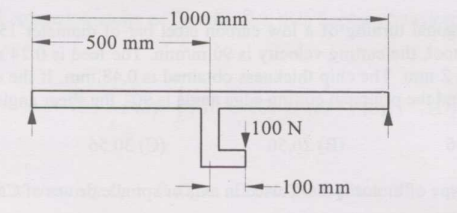
\includegraphics[width=0.5\textwidth]{fig.png} 
\end{figure}
\begin{multicols}{4}
    \begin{enumerate}
        \item $25$
        \item $30$
        \item $35$
        \item $60$
    \end{enumerate}
\end{multicols}
\bigskip
\item A ball bearing operating at a load F has 8000 hours of life. The life of the bearing, in hours, when the load is doubled to $2F$ is
\begin{multicols}{4}
    \begin{enumerate}
        \item $8000$
        \item $6000$
        \item $4000$
        \item $1000$
    \end{enumerate}
\end{multicols}
\bigskip
\item During inelastic collision of two particles, which one of the following is conserved?
\begin{enumerate}
        \item total linear momentum only
        \item total kinetic energy only
        \item both linear momentum and kinetic energy
        \item neither linear momentum nor kinetic energy 
\end{enumerate}
\bigskip
\item A steel rod of length L and diameter D, fixed at both ends, is uniformly heated to a temperature rise of $\Delta T$. The Young's modulus is E and the coefficient of linear expansion is a. The thermal stress in the rod is
\begin{multicols}{4}
    \begin{enumerate}
        \item $0$
        \item $\alpha\Delta T$
        \item $E\alpha\Delta T$
        \item $E\alpha\Delta TL$
    \end{enumerate}
\end{multicols}
\bigskip
\item For an underdamped harmonic oscillator, resonance

\begin{enumerate}
        \item occurs when excitation frequency is greater than undamped natural frequency
        \item occurs when excitation frequency is equal to undamped natural frequency
        \item occurs when excitation frequency is equal to undamped natural frequency
        \item never occurs
\end{enumerate}

\bigskip
\item If a particular Fe-C alloy contains less than $ 0.83\% $ carbon, it is called
\begin{multicols}{2}
    \begin{enumerate}
        \item high speed steel
        \item hypoeutectoid steel
        \item hypereutectoid steel
        \item cast iron
    \end{enumerate}
\end{multicols}
\bigskip
\item Which of the following engineering materials is the most suitable candidate for hot chamber die casting ?
\begin{multicols}{2}
    \begin{enumerate}
        \item low carbon steel 
        \item titanium 
        \item copper 
        \item tin
    \end{enumerate}
\end{multicols}
\bigskip
\item Which of the following is a solid state joining  process?
\begin{multicols}{2}
    \begin{enumerate}
        \item gas tungsten are welding
        \item resistance spot welding
        \item friction welding 
        \item submerged arc welding 
    \end{enumerate}
\end{multicols}

\end{enumerate}


\end{document}
